\documentclass[11pt,a4paper]{article}

% --- Core Typography & Encodings ---
\usepackage[utf8]{inputenc}
\usepackage[T1]{fontenc}
\usepackage{lmodern}            % High-quality scalable Latin Modern fonts
\usepackage{microtype}           % Improved optical margins, kerning, and font expansion

% --- Mathematical Packages ---
\usepackage{amsmath,amssymb,amsfonts,mathtools}
\usepackage{bm}

% --- Layout & Geometry ---
\usepackage{geometry}
\geometry{
    margin=0.9in,
    top=0.95in,
    bottom=0.95in,
    headheight=14pt,
    footskip=0.35in
}

% --- Colors & Styling ---
\usepackage{xcolor}
\definecolor{primarynavy}{RGB}{20, 45, 85}
\definecolor{accentcrimson}{RGB}{175, 35, 45}
\definecolor{darkslate}{RGB}{45, 55, 72}
\definecolor{softbluebg}{RGB}{246, 249, 254}
\definecolor{borderblue}{RGB}{180, 205, 235}
\definecolor{lightgrayline}{RGB}{220, 226, 235}

% --- Section Titles Styling ---
\usepackage{titlesec}
\titleformat{\section}
    {\color{primarynavy}\Large\bfseries}
    {\thesection}{0.8em}{}
    [{\color{lightgrayline}\titlerule[0.8pt]}]

\titleformat{\subsection}
    {\color{primarynavy}\large\bfseries}
    {\thesubsection}{0.6em}{}

% --- Running Headers & Footers ---
\usepackage{fancyhdr}
\pagestyle{fancy}
\fancyhf{}
\fancyhead[L]{\small\color{darkslate}\textit{Planck's Law of Blackbody Radiation}}
\fancyhead[R]{\small\color{darkslate}\nouppercase{\leftmark}}
\fancyfoot[C]{\small\color{darkslate}\thepage}
\renewcommand{\headrulewidth}{0.4pt}
\renewcommand{\footrulewidth}{0pt}

% --- Boxes & Environments ---
\usepackage{tcolorbox}

% Master Equation Result Box (Clean, Elegant, Publication-grade)
\newtcolorbox{resultbox}[1][]{
    colback=softbluebg,
    colframe=primarynavy,
    arc=2mm,
    boxrule=1.1pt,
    left=10pt,
    right=10pt,
    top=5pt,
    bottom=5pt,
    before=\vspace{0.3em}\noindent,
    after=\vspace{0.3em},
    #1
}

% Conceptual Postulate Box
\newtcolorbox{postulatebox}[1][]{
    colback=softbluebg!60,
    colframe=borderblue,
    arc=1.5mm,
    boxrule=0.8pt,
    left=9pt,
    right=9pt,
    top=5pt,
    bottom=5pt,
    before=\vspace{0.3em}\noindent,
    after=\vspace{0.3em},
    #1
}

% --- Tables & Lists ---
\usepackage{booktabs}
\usepackage{float}
\usepackage{enumitem}
\setlist{itemsep=3pt, topsep=4pt}

% --- Graphics & Plots ---
\usepackage{tikz}
\usetikzlibrary{arrows.meta, positioning, calc}

% --- Hyperlinks ---
\usepackage{hyperref}
\hypersetup{
    colorlinks=true,
    linkcolor=primarynavy,
    citecolor=primarynavy,
    urlcolor=primarynavy,
    hypertexnames=false,
    pdftitle={Planck's Law of Blackbody Radiation: Comprehensive Derivation and Limiting Cases},
    pdfauthor={Physics Lecture Notes}
}

% --- Custom Math Notation ---
\newcommand{\diff}{\mathrm{d}}
\newcommand{\kB}{k_{\mathrm{B}}}
\newcommand{\avgE}{\langle E \rangle}

\setlength{\parskip}{0.35em}
\setlength{\parindent}{0pt}
\setlength{\abovedisplayskip}{6pt plus 2pt minus 2pt}
\setlength{\belowdisplayskip}{6pt plus 2pt minus 2pt}
\setlength{\abovedisplayshortskip}{3pt plus 1pt minus 1pt}
\setlength{\belowdisplayshortskip}{3pt plus 1pt minus 1pt}

% =========================================================================
% DOCUMENT METADATA
% =========================================================================
\title{
    \vspace{-1.5cm}
    {\color{primarynavy}\Huge\bfseries Planck's Law of Blackbody Radiation}\\[0.35em]
    {\Large\color{darkslate} Quantum Hypothesis, Comprehensive Derivation, Limiting Cases, and Stefan--Boltzmann Law}
}
\author{\textbf{Physics Lecture Notes} \quad$\vert$\quad Advanced Modern Physics \& Thermodynamics}
\date{}

\begin{document}

\maketitle
\thispagestyle{plain}

\begin{abstract}
\noindent
This document presents a rigorous and pedagogical derivation of Max Planck's distribution law for blackbody radiation, thoroughly verified against foundational lecture notes. Starting from Planck's quantum postulate for cavity resonators and the Maxwell--Boltzmann energy distribution, we evaluate the discrete oscillator partition sums using generating functions. We determine the spectral radiant energy density in both frequency and wavelength domains, demonstrating how the quantum distribution resolves the classical ultraviolet catastrophe ($\lambda \to 0$). Furthermore, we establish the asymptotic convergence to the classical Rayleigh--Jeans law at long wavelengths and Wien's distribution at short wavelengths. Finally, by integrating over all frequencies, we rigorously deduce the Stefan--Boltzmann law ($J = \sigma T^4$) and calculate the exact analytical expressions and values for the radiation constant $a$ and Stefan's constant $\sigma$.
\end{abstract}

\vspace{0.5em}

% =========================================================================
% SECTION 1: PLANCK'S QUANTUM HYPOTHESIS
% =========================================================================
\section{Planck's Quantum Hypothesis}

In classical electrodynamics and thermodynamics, cavity radiation was assumed to exchange energy continuously with the material cavity walls. Applying the classical equipartition theorem to standing electromagnetic waves led directly to the Rayleigh--Jeans divergence, famously termed the \textit{ultraviolet catastrophe}.

In December 1900, Max Planck resolved this crisis by proposing that the material walls of a blackbody enclosure contain microscopic entities (atoms and molecules) acting as harmonic resonators (or oscillators):

\begin{postulatebox}
\textbf{Planck's Fundamental Postulates:}
\begin{enumerate}[label=(\roman*)]
    \item \textbf{Quantized Energy States:} The energy of any microscopic atomic resonator of natural frequency $\nu$ cannot take arbitrary continuous values. Instead, it is constrained to integral multiples of a fundamental energy quantum $\epsilon = h\nu$:
    \begin{equation}
        E_n = n h \nu, \quad n \in \{0, 1, 2, \dots\} \tag{I}
    \end{equation}
    where $h \approx 6.626 \times 10^{-34}\,\mathrm{J}\cdot\mathrm{s}$ denotes Planck's constant.
    \item \textbf{Discrete Radiation Exchange:} Energy is neither emitted nor absorbed continuously, but exclusively in discrete bundles (quanta), each bearing magnitude $\Delta E = h\nu$.
\end{enumerate}
\end{postulatebox}

According to the Maxwell--Boltzmann statistics, the thermal probability $P(E_n)$ that a resonator occupies the discrete energy level $E_n$ at absolute temperature $T$ is governed by the Boltzmann factor:
\begin{equation}
    P(E_n) \propto e^{-E_n / \kB T} = e^{-n h \nu / \kB T}
\end{equation}
The ensemble average energy $\bar{\epsilon} \equiv \avgE$ of an oscillator mode is computed via the expectation value:
\begin{equation}
    \bar{\epsilon} \equiv \avgE = \frac{\sum_{n=0}^{\infty} E_n \, e^{-E_n / \kB T}}{\sum_{n=0}^{\infty} e^{-E_n / \kB T}} \tag{II}
\end{equation}
Substituting $E_n = n h \nu$ yields:
\begin{equation}
    \bar{\epsilon} = \frac{\sum_{n=0}^{\infty} n h \nu \, e^{-n h \nu / \kB T}}{\sum_{n=0}^{\infty} e^{-n h \nu / \kB T}} \tag{III}
\end{equation}

% =========================================================================
% SECTION 2: EVALUATING THE DISCRETE SUMS
% =========================================================================
\section{Evaluating the Partition Sums}

To evaluate Eq.~(III) analytically, let us define the dimensionless parameter:
\begin{equation}
    x \equiv e^{-h\nu / \kB T} \quad (0 < x < 1 \text{ for } T > 0)
\end{equation}

\subsection{Denominator Sum}
The denominator represents the canonical partition function of a single oscillator, forming an infinite geometric series:
\begin{equation}
    \sum_{n=0}^{\infty} x^n = 1 + x + x^2 + x^3 + \dots = \frac{1}{1 - x} \quad (|x| < 1)
\end{equation}

\subsection{Numerator Sum}
The numerator series can be evaluated via differentiation with respect to $x$:
\begin{align}
    \sum_{n=0}^{\infty} n x^n &= x \sum_{n=0}^{\infty} n x^{n-1} 
    = x \frac{\diff}{\diff x}\left( \sum_{n=0}^{\infty} x^n \right) \notag \\
    &= x \frac{\diff}{\diff x}\left( \frac{1}{1 - x} \right) 
    = x \cdot \frac{1}{(1 - x)^2} = \frac{x}{(1 - x)^2}
\end{align}

\subsection{Average Energy per Oscillator}
Substituting the numerator and denominator expressions back into Eq.~(III):
\begin{equation}
    \bar{\epsilon} = \avgE = h\nu \cdot \frac{\dfrac{x}{(1 - x)^2}}{\dfrac{1}{1 - x}} = h\nu \cdot \frac{x}{1 - x}
\end{equation}
Dividing both the numerator and the denominator by $x$:
\begin{equation}
    \bar{\epsilon} = \frac{h\nu}{x^{-1} - 1}
\end{equation}
Since $x^{-1} = e^{h\nu / \kB T}$, we obtain Planck's celebrated expression for the mean thermal energy of a quantum oscillator:

\begin{resultbox}
\textbf{Planck Mean Oscillator Energy:}
\begin{equation}
    \boxed{\bar{\epsilon} \equiv \avgE = \frac{h\nu}{e^{\frac{h\nu}{\kB T}} - 1}} \tag{IV}
\end{equation}
\end{resultbox}
In contrast to the classical equipartition theorem which predicts an energy-independent value $\avgE_{\text{classical}} = \kB T$ for all frequencies, Eq.~(IV) shows that when $h\nu \gg \kB T$, the average energy drops exponentially toward zero.

% =========================================================================
% SECTION 3: SPECTRAL ENERGY DENSITY
% =========================================================================
\section{Spectral Radiant Energy Density}

The spectral energy density $u(\nu, T)\,\diff\nu$ represents the electromagnetic energy per unit volume in the frequency interval $[\nu, \nu + \diff\nu]$ at temperature $T$. In thermal equilibrium, the radiation field inside the cavity is in dynamic balance with the wall resonators.

Consequently, the energy density equals the product of the number of standing wave modes per unit volume, $g(\nu)\,\diff\nu$, and the average energy per mode, $\avgE$:
\begin{equation}
    u(\nu, T)\,\diff\nu = g(\nu) \avgE \,\diff\nu
\end{equation}

For a three-dimensional cavity of volume $V$, counting stationary electromagnetic modes with two independent transverse polarization states gives the density of modes:
\begin{equation}
    g(\nu)\,\diff\nu = \frac{8\pi \nu^2}{c^3}\,\diff\nu
\end{equation}
where $c$ is the speed of light in vacuum. Combining $g(\nu)\,\diff\nu$ with the average quantum energy $\avgE$ from Eq.~(IV):

\begin{resultbox}
\textbf{Planck Radiation Formula (Frequency Domain):}
\begin{equation}
    \boxed{u(\nu, T)\,\diff\nu = \frac{8\pi h \nu^3}{c^3} \frac{1}{e^{\frac{h\nu}{\kB T}} - 1} \,\diff\nu} \tag{V}
\end{equation}
\end{resultbox}

\subsection{Formulation in Terms of Wavelength (\texorpdfstring{$\lambda$}{lambda})}
Using the dispersion relation $\nu = \frac{c}{\lambda}$, we relate the differentials:
\begin{equation}
    \diff\nu = \left| -\frac{c}{\lambda^2} \,\diff\lambda \right| = \frac{c}{\lambda^2} \,\diff\lambda
\end{equation}
Equating the energy contained within corresponding spectral intervals, $u(\lambda, T)\,\diff\lambda = u(\nu, T)\,\diff\nu$:
\begin{align}
    u(\lambda, T)\,\diff\lambda &= \frac{8\pi h (c/\lambda)^3}{c^3} \frac{1}{e^{\frac{hc}{\lambda \kB T}} - 1} \left( \frac{c}{\lambda^2}\,\diff\lambda \right) \notag \\
    &= \frac{8\pi h c^3}{\lambda^3 c^3} \cdot \frac{c}{\lambda^2} \frac{1}{e^{\frac{hc}{\lambda \kB T}} - 1} \,\diff\lambda
\end{align}

Simplifying powers of $c$ and $\lambda$ yields the wavelength-dependent spectral density:

\begin{resultbox}
\textbf{Planck Radiation Formula (Wavelength Domain):}
\begin{equation}
    \boxed{u(\lambda, T)\,\diff\lambda = \frac{8\pi h c}{\lambda^5} \frac{1}{e^{\frac{hc}{\lambda \kB T}} - 1} \,\diff\lambda} \tag{VI}
\end{equation}
\end{resultbox}

% =========================================================================
% SECTION 4: LIMITING CASES & ASYMPTOTIC BEHAVIOR
% =========================================================================
\section{Limiting Cases and Physical Regimes}

To verify consistency with experimental laws and classical theory, we examine the three characteristic limiting regimes of Planck's distribution.

\subsection{Case 1: Short-Wavelength Limit and UV Catastrophe Resolution (\texorpdfstring{$\lambda \to 0$}{lambda -> 0})}
When the wavelength approaches zero ($\lambda \to 0$, or equivalently $\nu \to \infty$):
\begin{equation}
    \frac{hc}{\lambda \kB T} \to \infty \implies e^{\frac{hc}{\lambda \kB T}} \to \infty
\end{equation}
Because the denominator grows exponentially, it dominates the algebraic polynomial $\lambda^{-5}$ in the numerator:
\begin{equation}
    \lim_{\lambda \to 0} u(\lambda, T) = \lim_{\lambda \to 0} \frac{8\pi hc}{\lambda^5} e^{-\frac{hc}{\lambda \kB T}} = 0
\end{equation}
\begin{postulatebox}
\textbf{Physical Significance:} 
This mathematical result directly resolves the classical \textbf{``Ultraviolet Catastrophe''}. In classical physics, $u(\lambda, T) \propto \lambda^{-4}$, which diverges toward infinity as $\lambda \to 0$. In quantum theory, the discrete energy requirement $h\nu$ becomes so large compared to the available thermal energy $\kB T$ that high-frequency modes remain unexcited (frozen out).
\end{postulatebox}

\subsection{Case 2: Long-Wavelength Limit / Rayleigh--Jeans Law (\texorpdfstring{$\lambda \gg \frac{hc}{\kB T}$}{lambda >> hc/kT})}
When $\lambda \gg \frac{hc}{\kB T}$ (or $h\nu \ll \kB T$), the exponent is very small. We perform a Taylor series expansion of the exponential term:
\begin{equation}
    e^{\frac{hc}{\lambda \kB T}} = 1 + \frac{hc}{\lambda \kB T} + \frac{1}{2}\left( \frac{hc}{\lambda \kB T} \right)^2 + \dots \approx 1 + \frac{hc}{\lambda \kB T}
\end{equation}
Substituting this approximation into Eq.~(VI):
\begin{equation}
    u_\lambda(\lambda, T)\,\diff\lambda \approx \frac{8\pi hc}{\lambda^5} \frac{\diff\lambda}{\left(1 + \dfrac{hc}{\lambda \kB T}\right) - 1} 
    = \frac{8\pi hc}{\lambda^5} \left( \frac{\lambda \kB T}{hc} \right) \,\diff\lambda
\end{equation}

\begin{resultbox}
\textbf{Rayleigh--Jeans Distribution Law:}
\begin{equation}
    \boxed{u_\lambda(\lambda, T)\,\diff\lambda = \frac{8\pi \kB T}{\lambda^4} \,\diff\lambda} \tag{VII}
\end{equation}
\end{resultbox}
Planck's quantum formula smoothly recovers the classical Rayleigh--Jeans law in the domain where quantum discretization effects become negligible ($h\nu \ll \kB T$).

\subsection{Case 3: Short-Wavelength Limit / Wien's Distribution Law (\texorpdfstring{$\lambda \ll \frac{hc}{\kB T}$}{lambda << hc/kT})}
For $\lambda \ll \frac{hc}{\kB T}$ (or $h\nu \gg \kB T$), the exponential term is much greater than unity:
\begin{equation}
    e^{\frac{hc}{\lambda \kB T}} \gg 1 \implies e^{\frac{hc}{\lambda \kB T}} - 1 \approx e^{\frac{hc}{\lambda \kB T}}
\end{equation}
Substituting this approximation into Eq.~(VI) gives:
\begin{equation}
    u_\lambda(\lambda, T)\,\diff\lambda \approx \frac{8\pi hc}{\lambda^5} e^{-\frac{hc}{\lambda \kB T}} \,\diff\lambda
\end{equation}

\begin{resultbox}
\textbf{Wien's Distribution Law:}
\begin{equation}
    \boxed{u_\lambda(\lambda, T)\,\diff\lambda = \frac{A}{\lambda^5} e^{-\frac{B}{\lambda T}} \,\diff\lambda} \tag{VIII}
\end{equation}
\end{resultbox}
where $A = 8\pi hc$ and $B = \frac{hc}{\kB}$ represent Wien's empirical constants. Planck's law thus naturally reproduces Wilhelm Wien's semi-empirical formula at short wavelengths.

\begin{table}[H]
\centering
\footnotesize
\caption{Systematic Comparison of Blackbody Radiation Formulas}
\label{tab:comparison}
\vspace{0.3em}
\begin{tabular}{llll}
\toprule
\textbf{Theory / Law} & \textbf{Spectral Density $u(\lambda, T)$} & \textbf{Validity Regime} & \textbf{Physical Foundation} \\ \midrule
\textbf{Rayleigh--Jeans} & $\dfrac{8\pi \kB T}{\lambda^4}$ & Long $\lambda$ ($\lambda \kB T \gg hc$) & Classical Equipartition ($\avgE = \kB T$) \\[0.6em]
\textbf{Wien's Law}      & $\dfrac{8\pi hc}{\lambda^5} e^{-\frac{hc}{\lambda \kB T}}$ & Short $\lambda$ ($\lambda \kB T \ll hc$) & Empirical / Maxwellian tail \\[0.6em]
\textbf{Planck's Law}    & $\dfrac{8\pi hc}{\lambda^5} \dfrac{1}{e^{\frac{hc}{\lambda \kB T}} - 1}$ & Universal (All $\lambda, T$) & Energy Quantization ($E_n = nh\nu$) \\ \bottomrule
\end{tabular}
\end{table}

% =========================================================================
% SECTION 5: TOTAL ENERGY DENSITY
% =========================================================================
\section{Total Energy Density of Blackbody Cavity}

The total radiant energy density $u(T)$ inside the cavity is obtained by integrating the spectral energy density over all possible wavelengths from $\lambda = 0$ to $\lambda = \infty$:
\begin{equation}
    u(T) = \int_{0}^{\infty} u_\lambda(\lambda, T) \,\diff\lambda = \int_{0}^{\infty} \frac{8\pi hc}{\lambda^5} \frac{1}{e^{\frac{hc}{\lambda \kB T}} - 1} \,\diff\lambda
\end{equation}

\subsection{Transformation of Variables}
We introduce the dimensionless variable $x$:
\begin{equation}
    x \equiv \frac{hc}{\lambda \kB T} \implies \lambda = \frac{hc}{\kB T \, x}, \quad 
    \diff\lambda = -\frac{hc}{\kB T \, x^2} \,\diff x
\end{equation}
Evaluating the transformed integration limits:
\begin{equation}
    \lambda \to 0 \implies x \to \infty, \qquad \lambda \to \infty \implies x \to 0
\end{equation}
Substituting $\lambda$ and $\diff\lambda$ into the integral:
\begin{align}
    u(T) &= \int_{\infty}^{0} \frac{8\pi hc}{\left( \dfrac{hc}{\kB T \, x} \right)^5} \frac{1}{e^x - 1} \left( -\frac{hc}{\kB T \, x^2} \,\diff x \right) \notag \\
    &= \int_{\infty}^{0} \frac{8\pi hc (\kB T)^5 x^5}{(hc)^5} \frac{1}{e^x - 1} \left( -\frac{hc}{\kB T \, x^2} \,\diff x \right)
\end{align}
Reversing the limits of integration ($\int_{\infty}^0 \to \int_0^\infty$) absorbs the negative sign:
\begin{equation}
    u(T) = \frac{8\pi (\kB T)^4}{h^3 c^3} \int_{0}^{\infty} \frac{x^3}{e^x - 1} \,\diff x
\end{equation}

\subsection{Standard Bose--Einstein Integral}
The definite integral evaluates via the Riemann zeta function $\zeta(s)$ and gamma function $\Gamma(s)$:
\begin{equation}
    \int_{0}^{\infty} \frac{x^3}{e^x - 1} \,\diff x = \Gamma(4) \zeta(4) = 6 \left( \frac{\pi^4}{90} \right) = \frac{\pi^4}{15}
\end{equation}
Substituting this exact result yields:

\begin{resultbox}
\textbf{Total Cavity Energy Density:}
\begin{equation}
    \boxed{u(T) = \left[ \frac{8\pi^5 \kB^4}{15 h^3 c^3} \right] T^4 = a T^4} \tag{IX}
\end{equation}
\end{resultbox}
where $a$ is the \textit{radiation constant}:
\begin{equation}
    a \equiv \frac{8\pi^5 \kB^4}{15 h^3 c^3} \approx 7.5657 \times 10^{-16} \,\mathrm{J}\cdot\mathrm{m}^{-3}\cdot\mathrm{K}^{-4}
\end{equation}

\begin{postulatebox}
\textbf{Dimensional Analysis \& Units Verification:}
\begin{equation*}
    [u(T)] = \frac{\mathrm{J}}{\mathrm{m}^3}, \quad [T] = \mathrm{K} \implies [a] = \mathrm{J}\cdot\mathrm{m}^{-3}\cdot\mathrm{K}^{-4}
\end{equation*}
Noting that $1\,\mathrm{W} = 1\,\mathrm{J}\cdot\mathrm{s}^{-1}$, the radiation constant is dimensionally consistent across thermodynamic frameworks.
\end{postulatebox}

% =========================================================================
% SECTION 6: STEFAN-BOLTZMANN LAW
% =========================================================================
\section{Deduction of the Stefan--Boltzmann Law}

The total emissive power (or total radiant exitance) $J$ of a blackbody surface is defined as the total radiant energy emitted per unit surface area per unit time over all forward solid angles into a hemisphere ($2\pi$ steradians).

By integrating the isotropic photon flux leaving a small aperture of the cavity, the emitted flux $J$ is related to the internal energy density $u(T)$ by the geometric factor:
\begin{equation}
    J = \frac{c}{4} u(T)
\end{equation}
Substituting the derived formula for $u(T)$ from Eq.~(IX):
\begin{equation}
    J = \frac{c}{4} \left( \frac{8\pi^5 \kB^4}{15 h^3 c^3} \right) T^4 = \left( \frac{2\pi^5 \kB^4}{15 h^3 c^2} \right) T^4
\end{equation}

This rigorously derives the empirical \textbf{Stefan--Boltzmann Law}:

\begin{resultbox}
\textbf{Stefan--Boltzmann Law:}
\begin{equation}
    \boxed{J = \sigma T^4} \tag{X}
\end{equation}
\end{resultbox}
where \textbf{Stefan's constant} $\sigma$ is defined analytically in terms of fundamental physical constants:
\begin{equation}
    \sigma \equiv \frac{2\pi^5 \kB^4}{15 h^3 c^2} \approx 5.6704 \times 10^{-8} \,\mathrm{W}\cdot\mathrm{m}^{-2}\cdot\mathrm{K}^{-4}
\end{equation}
Expressed in base SI units:
\begin{equation}
    \sigma \approx 5.6704 \times 10^{-8} \,\mathrm{J}\cdot\mathrm{s}^{-1}\cdot\mathrm{m}^{-2}\cdot\mathrm{K}^{-4}
\end{equation}

% =========================================================================
% SECTION 7: COMPARATIVE SPECTRAL VISUALIZATION
% =========================================================================
\section{Comparison of Blackbody Spectra}

Figure~\ref{fig:spectra} provides a visual representation of Planck's quantum distribution alongside the classical Rayleigh--Jeans approximation and Wien's law, accurately replicating the comparative sketch from the lecture notes (Page~8 of manuscript).

\begin{figure}[H]
\centering
\vspace{-0.3em}
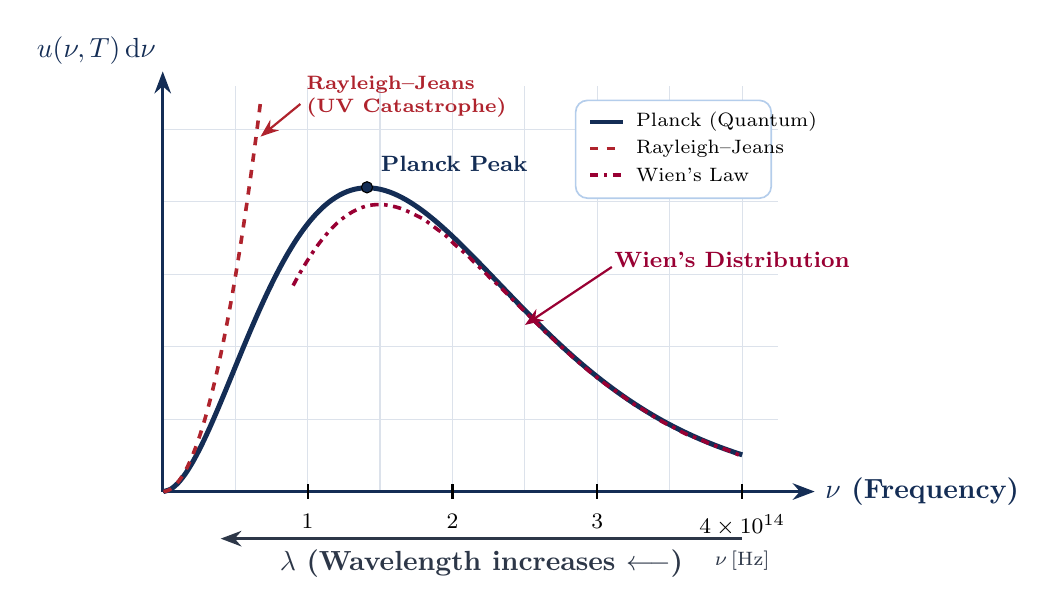
\begin{tikzpicture}[scale=0.92, >=Stealth]
    % Grid lines (subtle)
    \draw[lightgrayline, line width=0.4pt] (0,0) grid[xstep=1.0, ystep=1.0] (8.5, 5.6);

    % Main Axes
    \draw[->, line width=1.1pt, color=primarynavy] (0,0) -- (9.0,0) node[right] {\bfseries $\nu$ (Frequency)};
    \draw[->, line width=1.1pt, color=primarynavy] (0,0) -- (0,5.8) node[above left=-2pt] {\bfseries $u(\nu, T)\,\diff\nu$};

    % Reverse Wavelength Indicator Axis (matching Page 8 of lecture notes)
    \draw[<-, line width=1.0pt, color=darkslate] (0.8,-0.65) -- (8.0,-0.65) 
        node[midway, below] {\bfseries $\lambda$ (Wavelength increases $\longleftarrow$)};

    % Planck Curve (Smooth, peaking at x ~ 2.82, y ~ 4.20)
    \draw[line width=1.8pt, color=primarynavy, smooth] 
        plot[domain=0.01:8.0, samples=80] 
        (\x, {2.95 * (\x^3) / (exp(\x) - 1)});

    % Rayleigh-Jeans Divergence (Classical Ultraviolet Catastrophe: y = 2.95 * x^2)
    \draw[line width=1.3pt, dashed, color=accentcrimson, smooth] 
        plot[domain=0.01:1.35, samples=40] 
        (\x, {2.95 * \x^2});

    % Wien's Distribution Approximation (Matches high-frequency exponential tail: y = 2.95 * x^3 * e^-x)
    \draw[line width=1.3pt, dashdotted, color=purple!80!black, smooth] 
        plot[domain=1.8:8.0, samples=60] 
        (\x, {2.95 * (\x^3) * exp(-\x)});

    % Peak Annotation
    \draw[fill=primarynavy] (2.82, 4.20) circle (2.2pt);
    \node[color=primarynavy, font=\footnotesize\bfseries, above right=1pt] at (2.85, 4.25) {Planck Peak};

    % Catastrophe Annotation with Callout Arrow
    \draw[->, line width=0.8pt, color=accentcrimson] (1.9, 5.35) -- (1.35, 4.9);
    \node[color=accentcrimson, align=left, font=\scriptsize\bfseries, right] at (1.85, 5.45) 
        {Rayleigh--Jeans\\(\textbf{UV Catastrophe})};

    % Wien's Law Annotation with Arrow
    \draw[->, line width=0.8pt, color=purple!80!black] (6.2, 3.1) -- (5.0, 2.3);
    \node[color=purple!80!black, font=\footnotesize\bfseries, right] at (6.1, 3.2) 
        {Wien's Distribution};

    % Axis Ticks and Numeric Labels (matching Page 8 of lecture notes: 1, 2, 3, 4 x 10^14 Hz)
    \foreach \x/\label in {2/{1}, 4/{2}, 6/{3}, 8/{4 \times 10^{14}}} {
        \draw[line width=0.8pt] (\x, 0.1) -- (\x, -0.1) node[below=2pt, font=\footnotesize] {$\label$};
    }
    \node[below=18pt, font=\scriptsize\itshape, color=darkslate] at (8.0, 0) {$\nu\,[\mathrm{Hz}]$};

    % Legend Box
    \begin{scope}[shift={(5.7, 4.05)}]
        \draw[fill=white, draw=borderblue, rounded corners=1.5mm, line width=0.6pt] (0,0) rectangle (2.7, 1.35);
        \draw[line width=1.4pt, color=primarynavy] (0.2, 1.05) -- (0.65, 1.05);
        \node[right, font=\scriptsize] at (0.7, 1.05) {Planck (Quantum)};
        \draw[line width=1.1pt, dashed, color=accentcrimson] (0.2, 0.68) -- (0.65, 0.68);
        \node[right, font=\scriptsize] at (0.7, 0.68) {Rayleigh--Jeans};
        \draw[line width=1.1pt, dashdotted, color=purple!80!black] (0.2, 0.32) -- (0.65, 0.32);
        \node[right, font=\scriptsize] at (0.7, 0.32) {Wien's Law};
    \end{scope}

\end{tikzpicture}
\caption{Comparison of Blackbody Spectra: Spectral radiant energy density $u(\nu, T)$ as a function of frequency $\nu$ (pointing right) and wavelength $\lambda$ (pointing left), exactly reproducing the schematic layout in Page~8 of the foundational lecture notes. The classical Rayleigh--Jeans formula diverges quadratically ($\propto \nu^2$, red dashed curve), Wien's law captures the high-frequency exponential decay (purple dashdotted curve), and Planck's quantum law connects both asymptotic regimes seamlessly (blue solid curve).}
\label{fig:spectra}
\end{figure}

% =========================================================================
% SECTION 8: CONCLUSION
% =========================================================================
\section{Summary of Key Results}

The complete mathematical derivation confirms the following milestones:
\begin{enumerate}
    \item \textbf{Quantum Hypothesis:} The discretization of energy $E_n = nh\nu$ fundamentally replaces the continuous energy integral with a discrete geometric sum, leading directly to the quantum average oscillator energy $\avgE = \frac{h\nu}{e^{h\nu/\kB T} - 1}$.
    \item \textbf{Elimination of the UV Divergence:} The exponential denominator in Planck's formula ensures that as $\nu \to \infty$ ($\lambda \to 0$), the spectral energy density approaches zero, overcoming the classical failure.
    \item \textbf{Asymptotic Consistency:} Planck's law rigorously converges to the classical Rayleigh--Jeans law ($8\pi \kB T / \lambda^4$) in the long-wavelength limit and to Wien's law ($A\lambda^{-5} e^{-B/\lambda T}$) in the short-wavelength limit.
    \item \textbf{Stefan--Boltzmann Law:} Integrating $u(\nu, T)$ over all frequencies yields the exact $T^4$ dependence for both cavity energy density $u(T) = a T^4$ and total surface emissive power $J = \sigma T^4$, expressing the macroscopic radiation constants $a$ and $\sigma$ purely in terms of the fundamental constants $h, \kB, c,$ and $\pi$.
\end{enumerate}

\end{document}